\chapter{Model Selection and Hyperparameter Tuning}

\label{chap:ch3}

\quad In order to develop an accurate AI system for detecting depression from textual data, the choice of the right model and the fine-tuning of its parameters are critical steps. This chapter describes the process of selecting Random Forest as the preferred model. Known for its ability to handle complex datasets, Random Forest stands out as a powerful tool among machine learning algorithms.

\section{Reasoning Behind Choosing Random Forest}

In machine learning, selecting the most appropriate algorithm is very important to the success of any classifying task. This is also true in the case of depression detection, where the complexity and variability of the data demand an approach that is not only accurate but also can work on texts from different cultures. Looking at a  comprehensive study that evaluated twelve distinct machine learning algorithms across seven datasets\cite{siraj2023performanceModelComparison}, it was decided to use Random Forest (RF) as the AI model.

The study \cite{siraj2023performanceModelComparison} in question compared the performance of several algorithms, including Naive Bayes (NB), Linear Discriminant Analysis (LDA), Logistic Regression (LR), Artificial Neural Networks (ANN), Support Vector Machines (SVM), K-Nearest Neighbors (K-NN), Hoeffding Tree (HT), Decision Tree (DT), C4.5, Classification and Regression Tree (CART), Random Forest (RF), and Bayesian Belief Networks (BB), across multiple metrics. Among these, Random Forest showed the most consistent and high results, showing superior accuracy, precision, and Matthew’s Correlation Coefficient (MCC). Following Random Forest, the algorithms of Neural Networks (NN), Naive Bayes (NB), Bayesian Belief Networks (BB), and Logistic Regression (LR) were identified as the next most effective, in descending order of accuracy.

The study \cite{siraj2023performanceModelComparison} also highlighted the significance of the kappa statistic and Root Mean Square Error (RMSE) as important factors in assessing model performance, further validating the consistency of Random Forest in handling diverse and complex datasets. With these statistics, and in accordance with the study’s conclusion, the selection of Random Forest is motivated by its results across multiple validation metrics.

The datasets utilized for the comparative study are varied, each with its unique characteristics and relevance to different classification tasks:
\begin{itemize}
 
\item Breast Cancer Wisconsin (Original): This dataset contains 11 attributes and is used for binary classification (two classes) with 699 instances. It does include missing values, which would require additional preprocessing steps.

\item Statlog (Vehicle Silhouettes): Comprising 19 attributes over 846 instances, this dataset is for multiclass classification with four distinct classes and has no missing values.

\item Vertebral Column: With 7 attributes and 310 instances, this dataset is also used for multiclass classification, distinguishing among three classes, without any missing values.

\item Breast Tissue: This dataset has 10 attributes across 106 instances and is used for a more complex multiclass classification task with six classes, also free of missing values.

\item Contraceptive Method Choice: It includes 10 attributes and a larger number of instances at 1473. It’s structured for multiclass classification into three classes, and there are no missing values.

\item Image Segmentation: This is a sizable dataset with 20 attributes and 2310 instances for multiclass classification involving seven classes, and it contains no missing values.

\item Artificial Characters: The largest among the datasets listed, it boasts 8 attributes across a substantial 10218 instances. It’s designed for a multiclass classification with ten classes, and like most others here, it lacks missing values.

\end{itemize}

In the context of this study focused on depression detection, the dataset resembles the Breast Cancer Wisconsin dataset, because the model is also a binary classifier. However, the model differentiates itself with a higher dimensionality, processing 119 input attributes, which poses a greater complexity in feature representation and selection. For this dataset (Random Forest) RF achieved the highest accuracy at 97.85\%, suggesting it was the most successful in correctly identifying cases of breast cancer. It also had the highest kappa value of 95.03\%. Precision with RF was great as well, hitting a high of 98\%, while its recall was nearly as impressive at 97.9\%, showing its ability to identify most of the positive cases. 


Across the rest of the datasets analyzed in the study \cite{siraj2023performanceModelComparison}, Random Forest (RF) consistently was one of the best algorithms. Its F-measure and Matthew's Correlation Coefficient (MCC) values were notably high, often outperforming other algorithms. For instance, RF attained an accuracy of 98.48\%, kappa value of 98.23\%, and precision and recall rates both at 98.5\% on certain datasets, alongside a specificity of up to 99.7%.

While K-NN and Logistic Regression (LR) also demonstrated strong performances in certain cases, with K-NN leading in precision and recall in the Breast Tissue dataset and LR excelling with the highest MCC values for the Vehicle and Vertebral Column datasets, RF's overall dominance was clear. RF's ability to achieve the lowest error rates, coupled with the lowest root mean square error in the majority of datasets, further confirms its reliability as an algorithm for complex predictive tasks, including depression detection.

\section{Evaluation Metrics}
\quad Metrics are a crucial part of evaluating the effectiveness of a binary classifier. It's important to use a variety of tools and methods to understand different aspects of the model's performance. Here the metrics that were chosen for the evaluation of the depression binary classifier:

\begin{itemize}
    \item \textbf{Classification Metrics}: These include accuracy, precision, recall, and the F1-score, which together provide a comprehensive overview of overall model performance. Their respective equations are detailed, where TP are true positives, TN are true negatives, FP are false posivites and FN are false False Negatives.
    \begin{itemize}
        \item \textbf{Accuracy} measures the overall correctness of the model across all predictions \ref{accuracy}. 
        \item \textbf{Precision} assesses how many of the positively predicted cases were actually positive \ref{precision}.
        \item \textbf{Recall} (or sensitivity) determines how many of the actual positive cases were correctly identified by the model \ref{recall}.
        \item \textbf{F1-Score} is the harmonic mean of precision and recall, helping balance the two in scenarios where one may be more important than the other \ref{f1}.
        
        \begin{align} 
            &\mathit{Accuracy} = \frac{TP+TN}{TP+TN+FP+FN} \label{accuracy}\\
            &\mathit{Precision} = \frac{TP}{TP+FP} \label{precision}\\
            &\mathit{Recall} = \frac{TP}{TP+FN} \label{recall}\\
            &F1-Score = \frac{2*\mathit{Precision}*\mathit{Recall}}{\mathit{Precision}+\mathit{Recall} \label{f1}}
        \end{align}
    \end{itemize}
    \item \textbf{Confusion Matrix}: This is a table that visualizes the performance of the binary classifier by showing the actual versus predicted classifications. It helps identify the kinds of errors the model is making, such as confusing one class for another.
    \item \textbf{ROC Curve}: This graph shows the ability of the model to distinguish between the two classes at various threshold levels. It plots the true positive rate against the false positive rate, providing insight into the trade-offs between capturing positives and avoiding false alarms \cite{hoo2017roc}.
    \item \textbf{Feature Importance}: This metric highlights which inputs or variables in your data have the most influence on the model’s predictions. Understanding feature importance can help in refining the model by focusing on the most relevant factors.
\end{itemize}

By using these metrics, a detailed understanding of your model's strengths and weaknesses can be achieved, guiding improvements and ensuring it performs well across various conditions.

\section{Model Training Approach}

\quad To achieve an optimal model, it is essential to explore various training methodologies. This section describes the procedures followed in training the model.

\subsection{Initial Model Training Strategy}

\quad In the initial training phase, all available features were utilized without any adjustments to hyperparameters. The default settings of the Random Forest Classifier from sklearn were applied \cite{sklearn_api}. The dataset was partitioned in a 75/25 train/test split, ensuring an equal distribution of positive and negative cases by using the stratify option, as illustrated in Figure \ref{codeTrainRF}.

\begin{figure}[htbp]
	\centering
		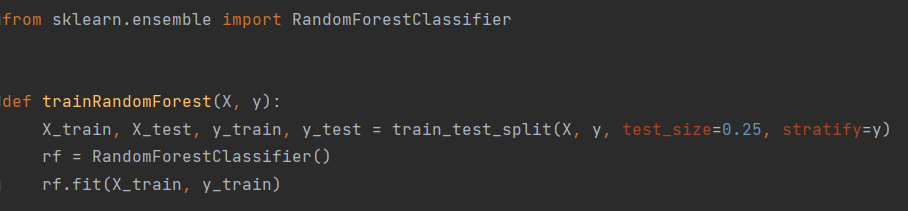
\includegraphics[scale=0.6]{LaTeX Bachelor Thesis Depression Signs Detection/figures/codeTrainingRF.png}
	\caption{Python code used for the initial training of the Random Forest Classifier}
	\label{codeTrainRF}
\end{figure}

The first experiment's results reveal a strong performance across the chosen metrics. The Classification Metrics plot shows high values for Accuracy (0.96), Precision (0.99), Recall (0.93), and F1 Score (0.96), indicating an efficient model with a balanced approach to both relevance (precision) and completeness (recall) \ref{classificationMetricsFirstExperiment}.

\begin{figure}[htbp]
	\centering
		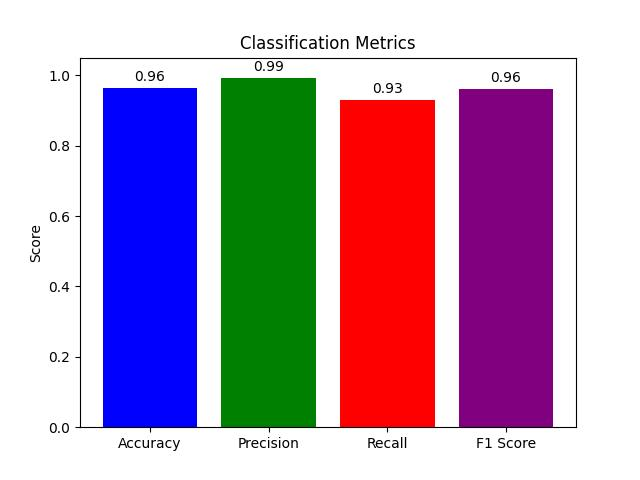
\includegraphics[scale=0.8]{LaTeX Bachelor Thesis Depression Signs Detection/figures/metrics/experiment1English/classificationMetrics.jpg}
	\caption{Classification Metrics First Experiment}
	\label{classificationMetricsFirstExperiment}
\end{figure}

The Confusion Matrix provides a visual confirmation of the model's performance, with a high number of true positives (891) and true negatives (969), and relatively few false positives (6) and false negatives (67) \ref{confusionMatrixFirstExperiment}. This suggests the model has more problems when finding depression.

\begin{figure}[htbp]
	\centering
		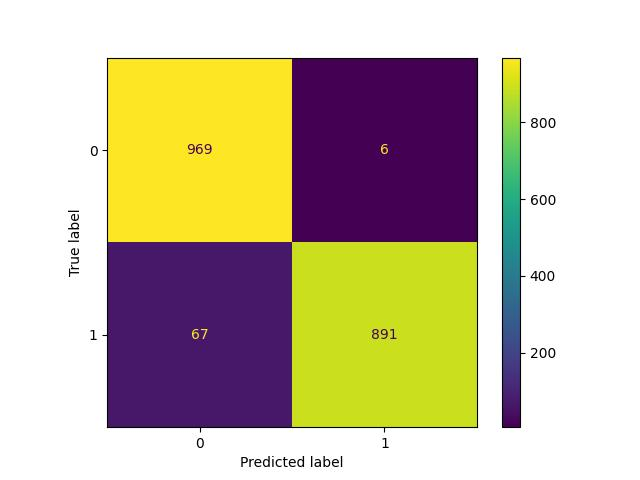
\includegraphics[scale=0.8]{LaTeX Bachelor Thesis Depression Signs Detection/figures/metrics/experiment1English/confusionMatrix.jpg}
	\caption{Confusion Matrix First Experiment}
	\label{confusionMatrixFirstExperiment}
\end{figure}

Looking at the ROC Curve, the model demonstrates an excellent ability to distinguish between the classes, as evidenced by the area under the curve (AUC) being close to 1 (0.99) \ref{rocCurveFirstExperiment}. This suggests that the model has a good discrimination capability with a high true positive rate and a low false positive rate across different thresholds.

\begin{figure}[htbp]
	\centering
		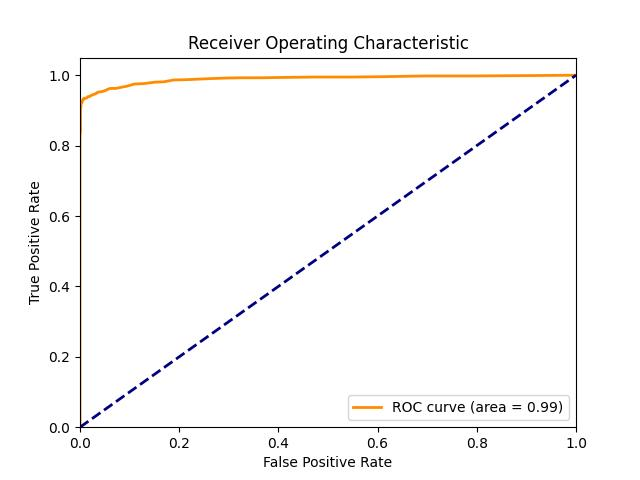
\includegraphics[scale=0.8]{LaTeX Bachelor Thesis Depression Signs Detection/figures/metrics/experiment1English/roc_curve.jpg}
	\caption{ROC Curve First Experiment}
	\label{rocCurveFirstExperiment}
\end{figure}

The Top 10 Feature Importances plot indicates which features have the most influence on the model's predictions. The leading features, labeled as 'WC' (Word Count) and 'WPS' (Words per Sentence), seem to be the most significant drivers, with the others contributing to varying lesser degrees \ref{top10FeaturesFirstExperiment}. This shows us that the length of the given text is very important in order for the model to give an accurate prediction.

\begin{figure}[htbp]
	\centering
		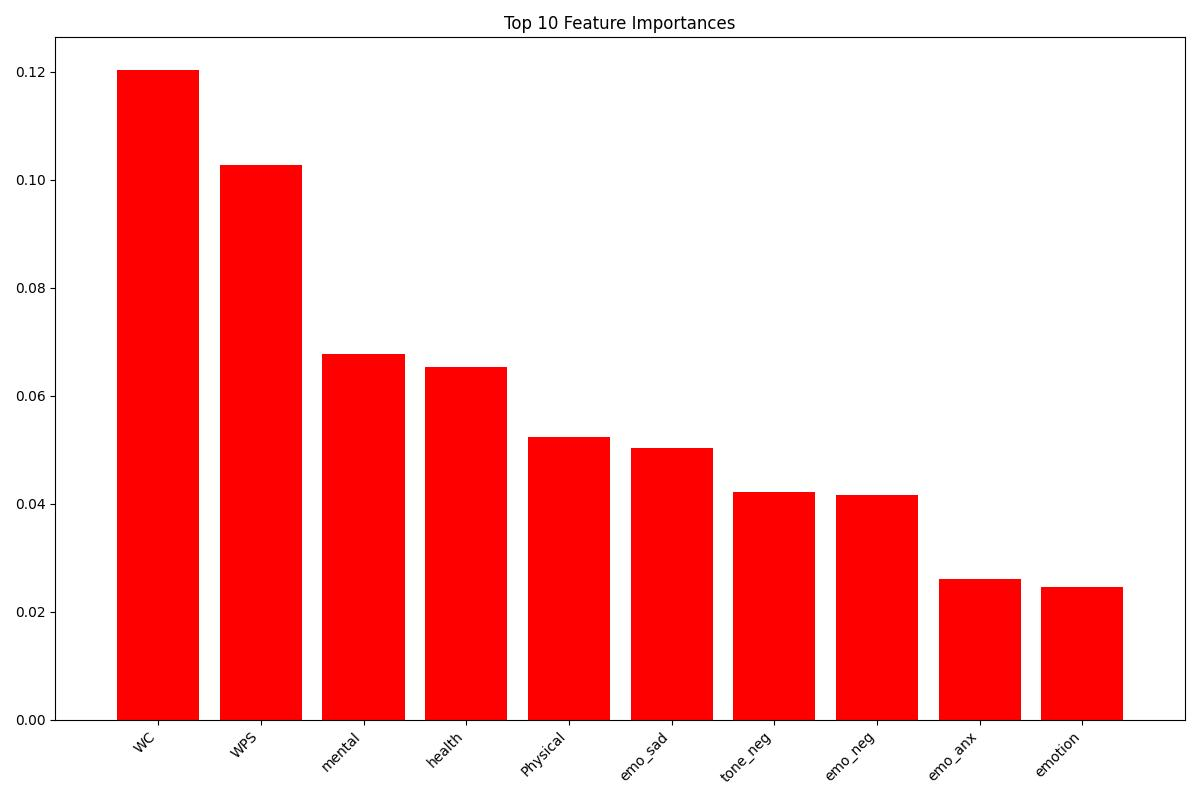
\includegraphics[scale=0.5]{LaTeX Bachelor Thesis Depression Signs Detection/figures/metrics/experiment1English/top10features.jpg}
	\caption{Top 10 Feature Importances First Experiment}
	\label{top10FeaturesFirstExperiment}
\end{figure}

Overall, the model appears to be highly effective, with strong performance indicators, which seems to be the result of the analysis done for choosing the pre-processing methods and classifier, namely LIWC \cite{boyd2022development} and Random Forrest.

\subsection{Hyperparameter Tuning}
The selection of Random Forest hyperparameters is guided by the study \cite{probst2019hyperparameters}. The adjusted hyperparameters are:

\begin{itemize}
  \item \textbf{mtry}: This represents the number of features considered for splitting at each node. Lower values promote tree diversity and are beneficial when there are many relevant predictors. Given the large feature set, a value lower than the default square root of the number of features is suggested to prevent dominant features from overshadowing others.
  \item \textbf{Number of Trees}: A sufficient number of trees ensures stable predictions and importance estimates. While more trees generally improve model performance, beyond a certain point the marginal gains diminish. For practical purposes, between 500 to 1000 trees are recommended.
  \item \textbf{Node Size}: The node size controls the depth of the tree. Smaller node sizes can potentially lead to over-fitting, particularly when the number of features is high. A larger than 1 node size is preferred to mitigate this risk and improve computational efficiency.
  \item \textbf{Sample Size}: The proportion of data used for training each tree. Smaller sample sizes lead to more diversity but can decrease individual tree accuracy. Optimal sample size needs to be problem-specific but sampling a subset, such as between 20\% and 90\% of the data, can yield good results while reducing runtime. 
\end{itemize}

These hyperparameters were tuned using Sequential Model-Based Optimization (SMBO) to determine their optimal values while considering the Area Under the ROC Curve (AUC) as the performance metric \cite{probst2019hyperparameters}.

For the depression binary classifier multiple configurations were tested. It was noticed that the optimal ranges for the hyperparameters were:
\begin{itemize}
    \item \textbf{mtry}: between 6 and 10
    \item \textbf{Number of trees}: between 700 and 1000
    \item \textbf{Node Size}: between 3 and 9
    \item \textbf{Sample size}: between 6 and 9
\end{itemize}

After training with all combinations of the mentioned ranges, the one who got the best results was 6 for mtry, 900 for number of trees, 3 for node size and 8 for sample size. The same metrics as in the first experiment were used to analyze the performance of the model and improvements were seen. For the classification metrics accuracy(0.97) has improved by 0.01, precision stayed the same, recall(0.96) was the one who improved the most by 0.03, and F1-score(0.97) improved by 0.01. These values can be seen comparing Figure \ref{classificationMetricsFirstExperiment}, which shows the classification metrics for the first experiment, with Figure \ref{classificationMetricsSecondExperiment}, which shows them for the second experiment. This shows that because of hyperparameters tuning, it succeeded in improving the part where the model from the first experiment lacked.

\begin{figure}[htbp]
	\centering
		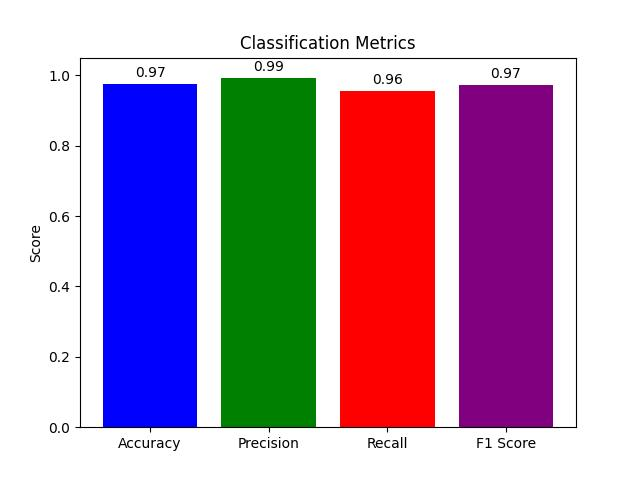
\includegraphics[scale=0.8]{LaTeX Bachelor Thesis Depression Signs Detection/figures/metrics/experiment2English/classificationMetrics.jpg}
	\caption{Classification Metrics Second Experiment}
	\label{classificationMetricsSecondExperiment}
\end{figure}

In the case of the confusion matrix for the second experiment \ref{confusionMatriSecondExperiment} it can be discovered that in comparison with the one for the first experiment \ref{confusionMatrixFirstExperiment}, as can the improvement of recall also tell, the values of the false positives decreased, from 67 to 43.

\begin{figure}[htbp]
	\centering
		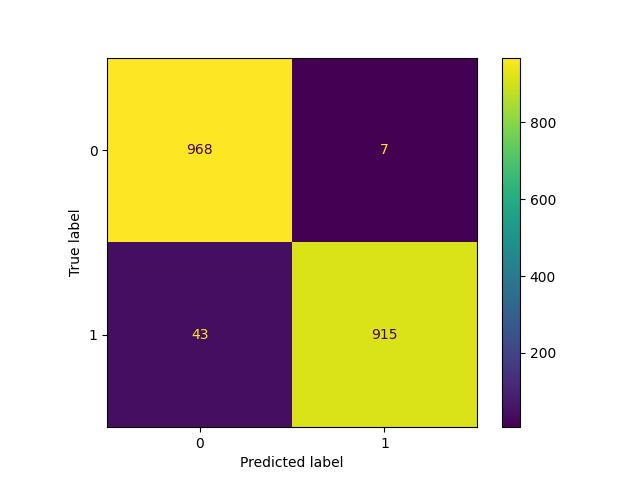
\includegraphics[scale=0.8]{LaTeX Bachelor Thesis Depression Signs Detection/figures/metrics/experiment2English/confusionMatrix.jpg}
	\caption{Confusion Matrix Second Experiment}
	\label{confusionMatriSecondExperiment}
\end{figure}

For the ROC curve for this experiment \ref{rocCurveSecondExperiment}, the area stayed the same when looking to the first two digits, but an improvement of the true positive rate can be noticed from the initial experiment \ref{rocCurveFirstExperiment}.

\begin{figure}[htbp]
	\centering
		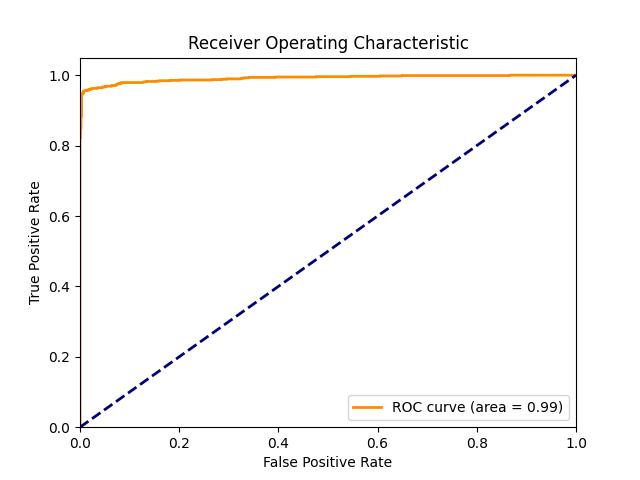
\includegraphics[scale=0.8]{LaTeX Bachelor Thesis Depression Signs Detection/figures/metrics/experiment2English/roc_curve.jpg}
	\caption{ROC Curve Second Experiment}
	\label{rocCurveSecondExperiment}
\end{figure}

Seeing the top 10 features of the second experiment \ref{top10FeaturesSecondExperiment}, it was noticed that in comparison with the initial one \ref{top10FeaturesFirstExperiment} that even though WC (Word Count) and WS (Words per Sentence) are the still the most important features, they are now by much less, from 0.12 and 0.10 to both being at 0.09. This shows that now there are more features taken into account when the model makes the classification and each is more influential. Also it is remarked that a feature in the first ten was changed, namely emo\_anx (anxiety) with cause (causation).

\begin{figure}[htbp]
	\centering
		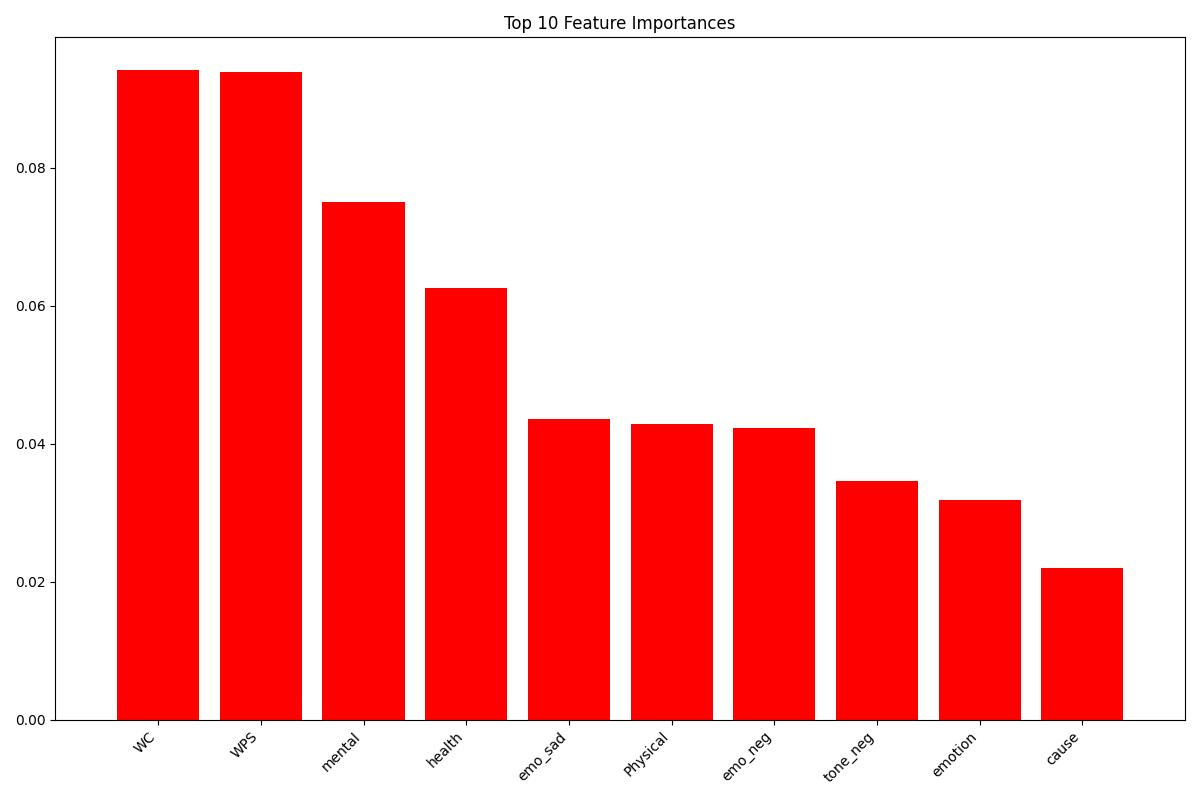
\includegraphics[scale=0.5]{LaTeX Bachelor Thesis Depression Signs Detection/figures/metrics/experiment2English/top10features.jpg}
	\caption{Top 10 Feature Importances Second Experiment}
	\label{top10FeaturesSecondExperiment}
\end{figure}



